\subsubsection{Denoiser}
We tried to replicate the training procedure stated in \cite{defossez2020} for the Denoiser model based on DEMUCS architecture \cite{demucs}. We used 100 hours of the DNS 2020 dataset \cite{reddy2020} for training, and its corresponding test set was used for testing.

\textbf{Architecture:} The depth of the encoder or the decoder is D = 5. Each encoder/decoder layer has hidden dimension H = 48, stride S = 4, and kernel size K = 8. These parameters were adapted from the original paper.

\textbf{Optimization:} The model was trained for 28K steps with a batch size of 7. The Adam \cite{kingma2017adam} optimizer was used with a learning rate of $3\times 10^{-4}$ with a Linear Warmup Cosine Decay and beta values of 0.9 and 0.999. The loss functions used were L1 loss and Multi Resolution STFT loss.
The model was trained on a 2 NVIDIA Tesla T4 GPUs. The training took 24 hours to complete. The training loss is shown in Figure \ref{fig:denoiser-training} and metrics on the test set are shown in Table \ref{tab:denoiser-test}.

\begin{figure}[h]
    \centering
    \begin{subfigure}{.3\textwidth}
      \centering
      % include first image
      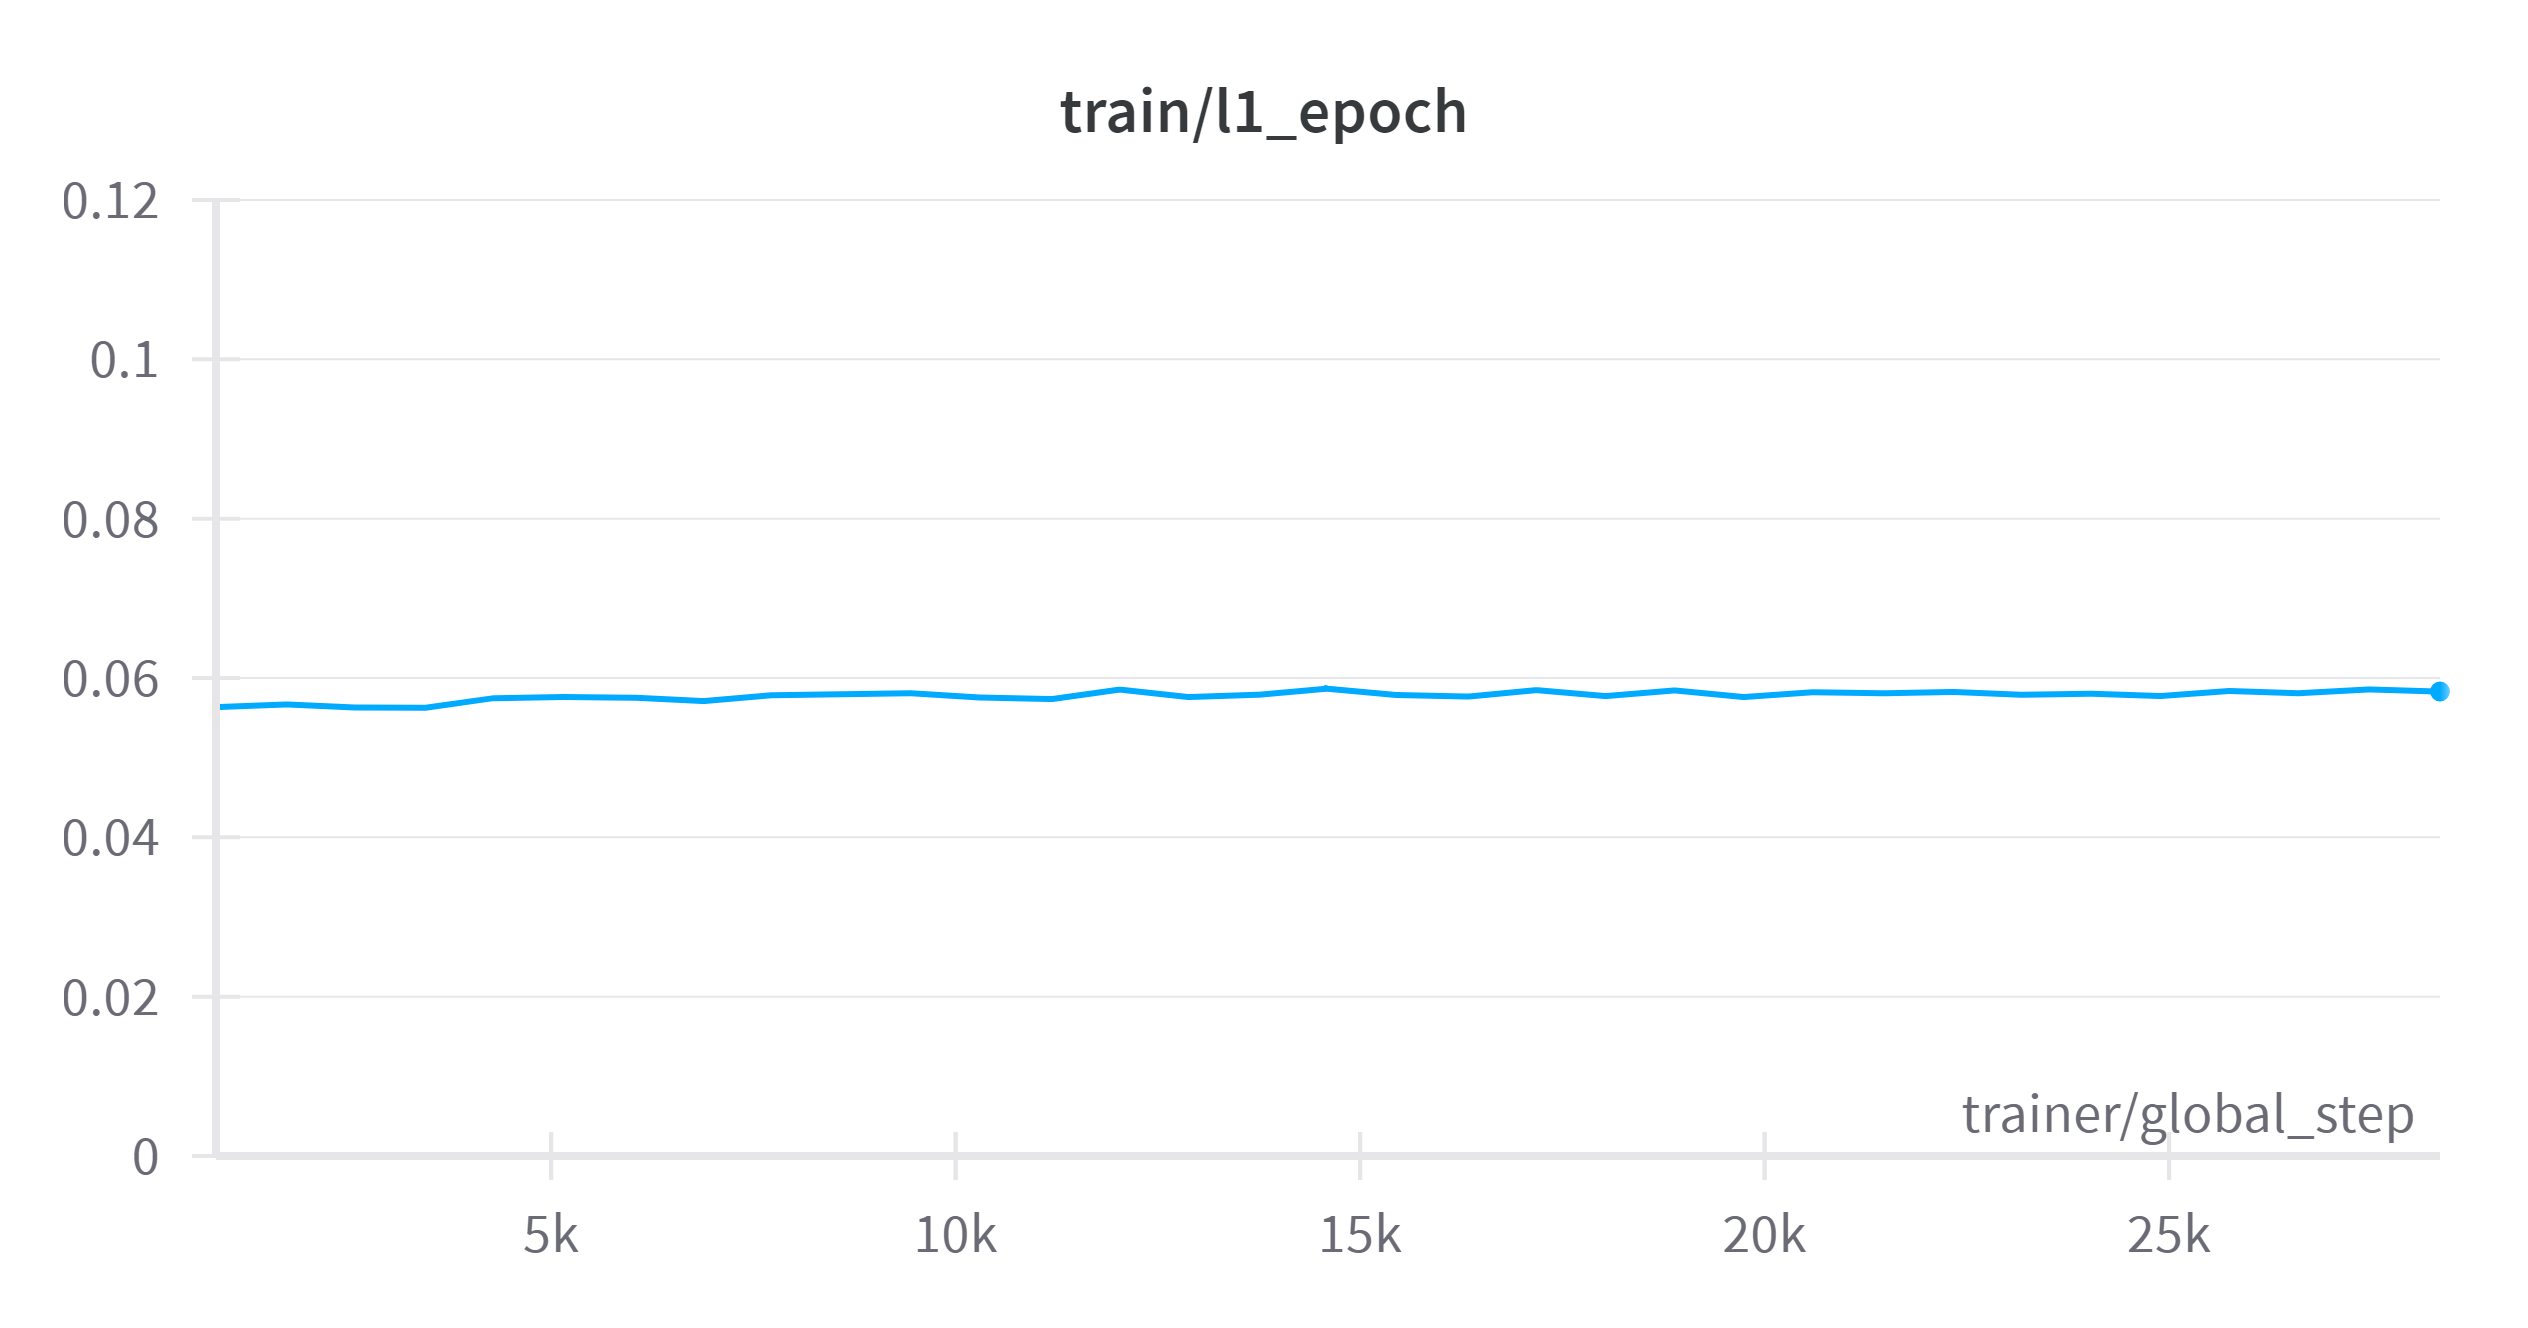
\includegraphics[width=1\linewidth]{images/experiments/denoiser/denoiser_DNS100hrs_train_l1.png}  
      \caption{L1 loss reported on\\ training set.}
      \label{fig:denoiser_train_l1}
    \end{subfigure}
    \begin{subfigure}{.3\textwidth}
      \centering
      % include second image
      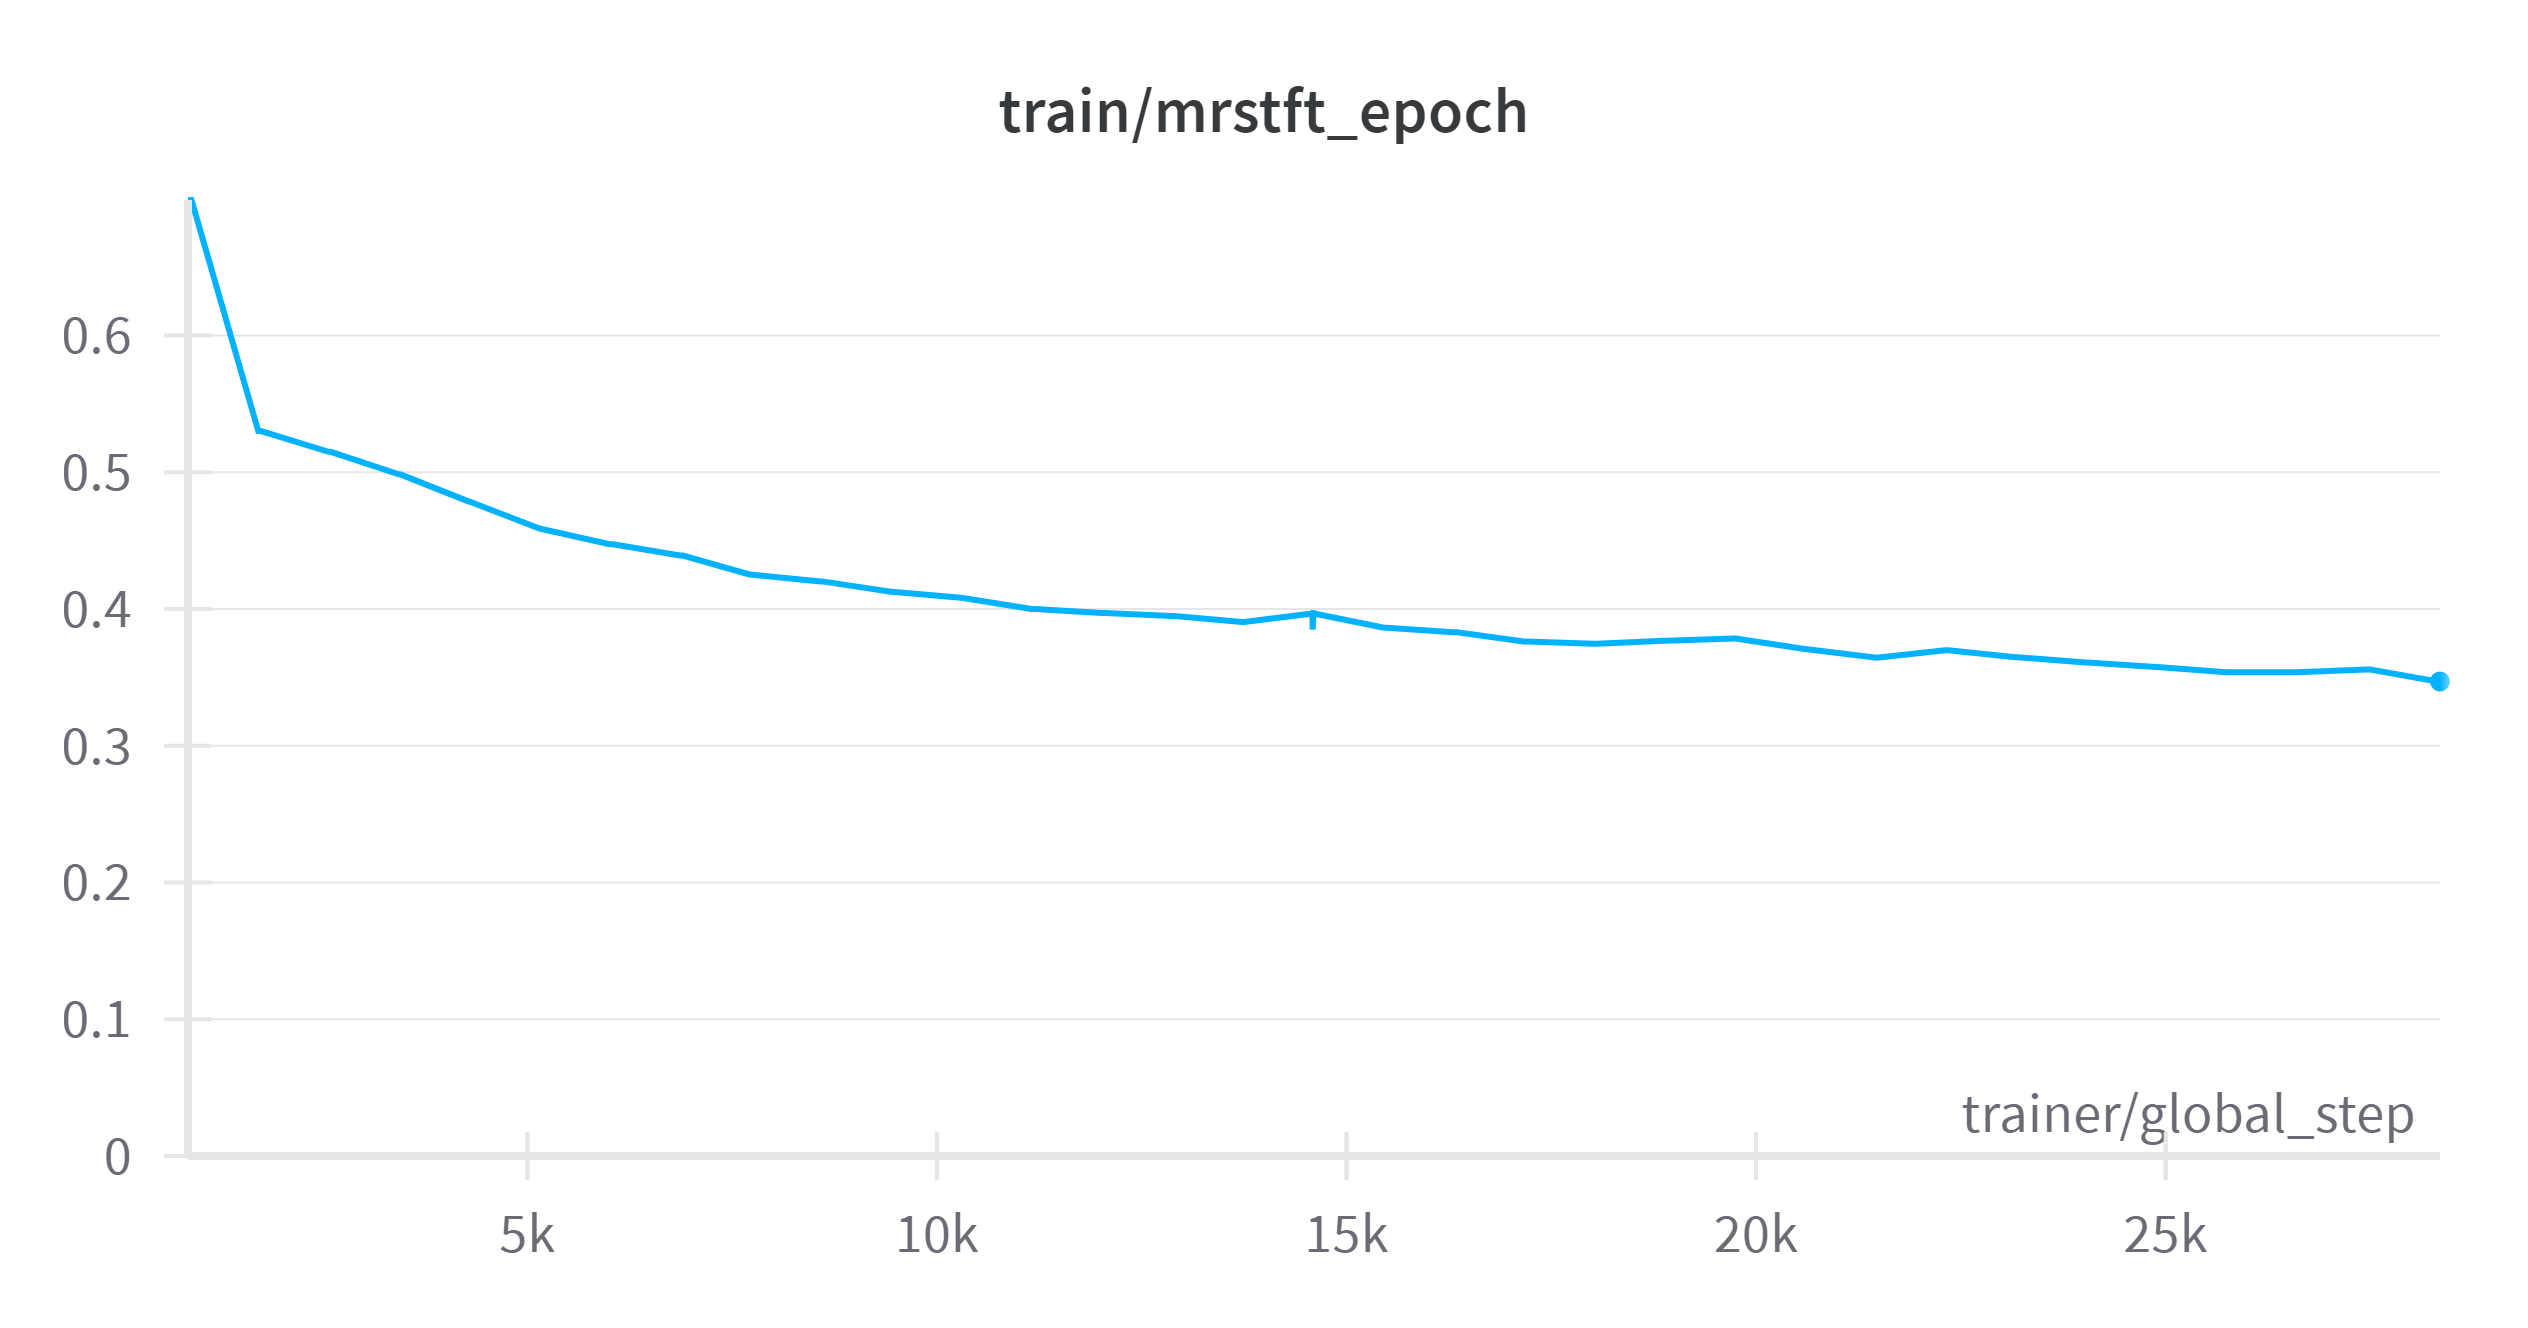
\includegraphics[width=1\linewidth]{images/experiments/denoiser/denoiser_DNS100hrs_train_mrstft.png}  
      \caption{MRSTFT loss reported on \\ training set.}
      \label{fig:denoiser_train_stft}
    \end{subfigure}
    \begin{subfigure}{.3\textwidth}
        \centering
        % include second image
        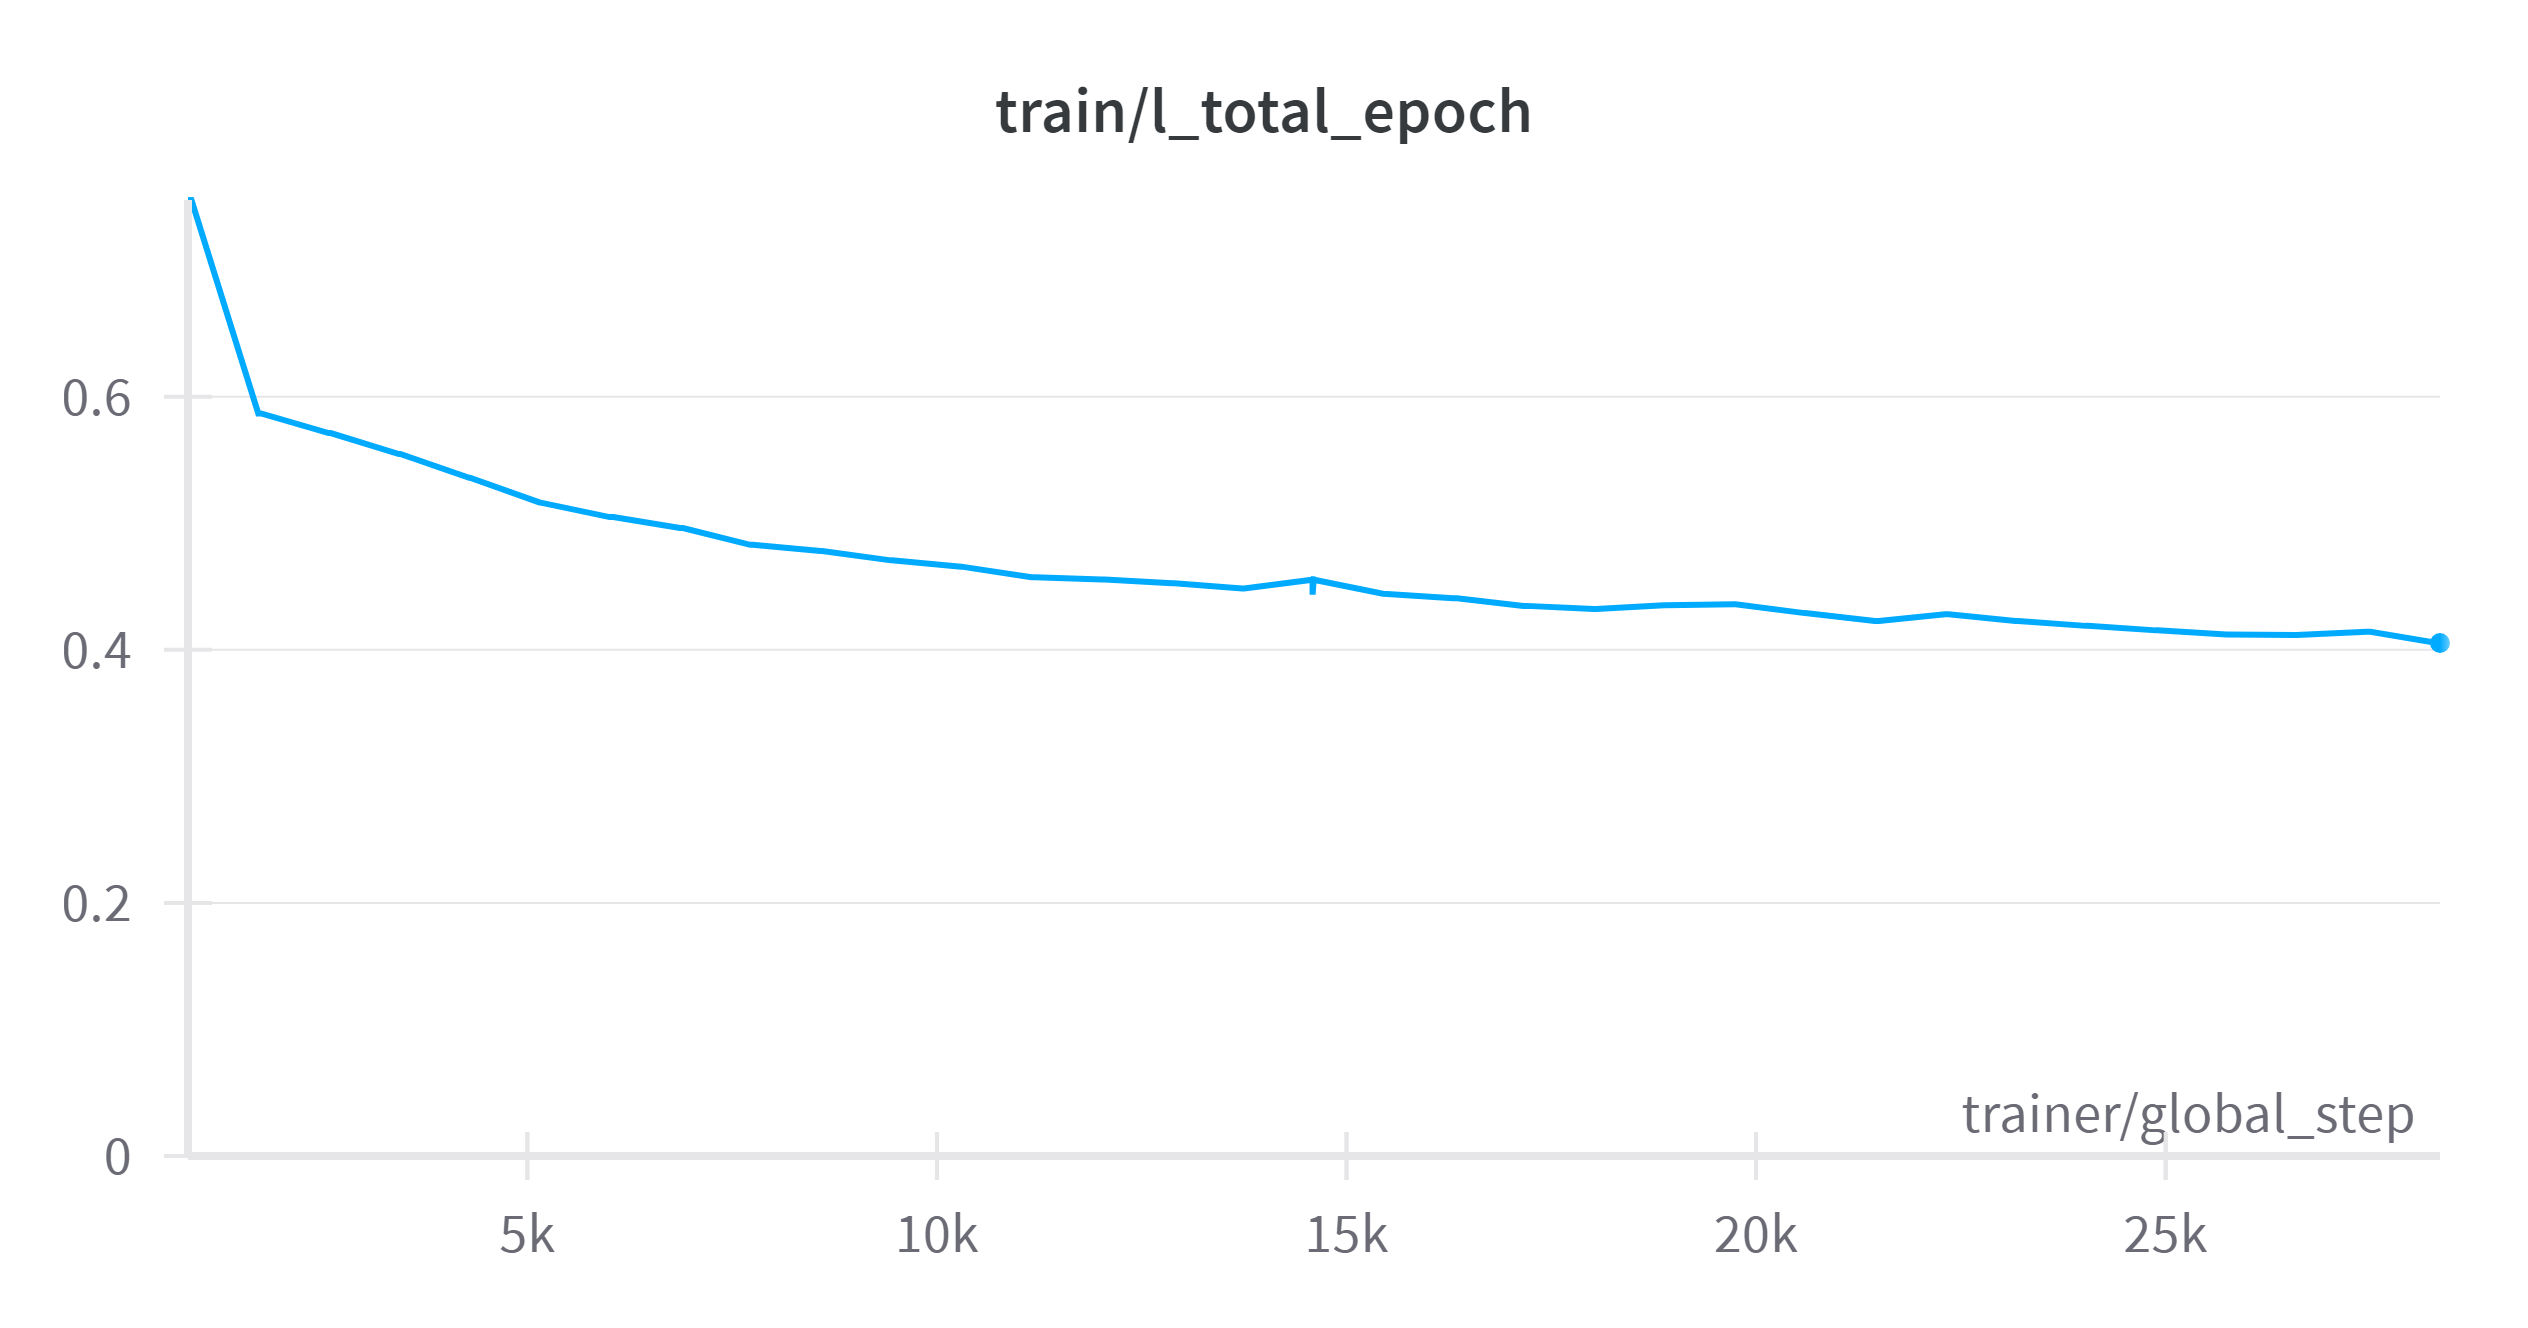
\includegraphics[width=1\linewidth]{images/experiments/denoiser/denoiser_DNS100hrs_train_total.png}  
        \caption{Total loss reported on\\ training set.}
        \label{fig:denoiser_train_total}
      \end{subfigure}


    % \newline


    % \begin{subfigure}{.3\textwidth}
    %   \centering
    %   % include third image
    %   \includegraphics[width=1\linewidth]{images/experiments/denoiser/denoiser_dns100hrs_val_stoi.png}  
    %   \caption{STOI reported on\\ test set.}
    %   \label{fig:denoiser_val_stoi}
    % \end{subfigure}
    % \begin{subfigure}{.3\textwidth}
    %     \centering
    %     % include fourth image
    %     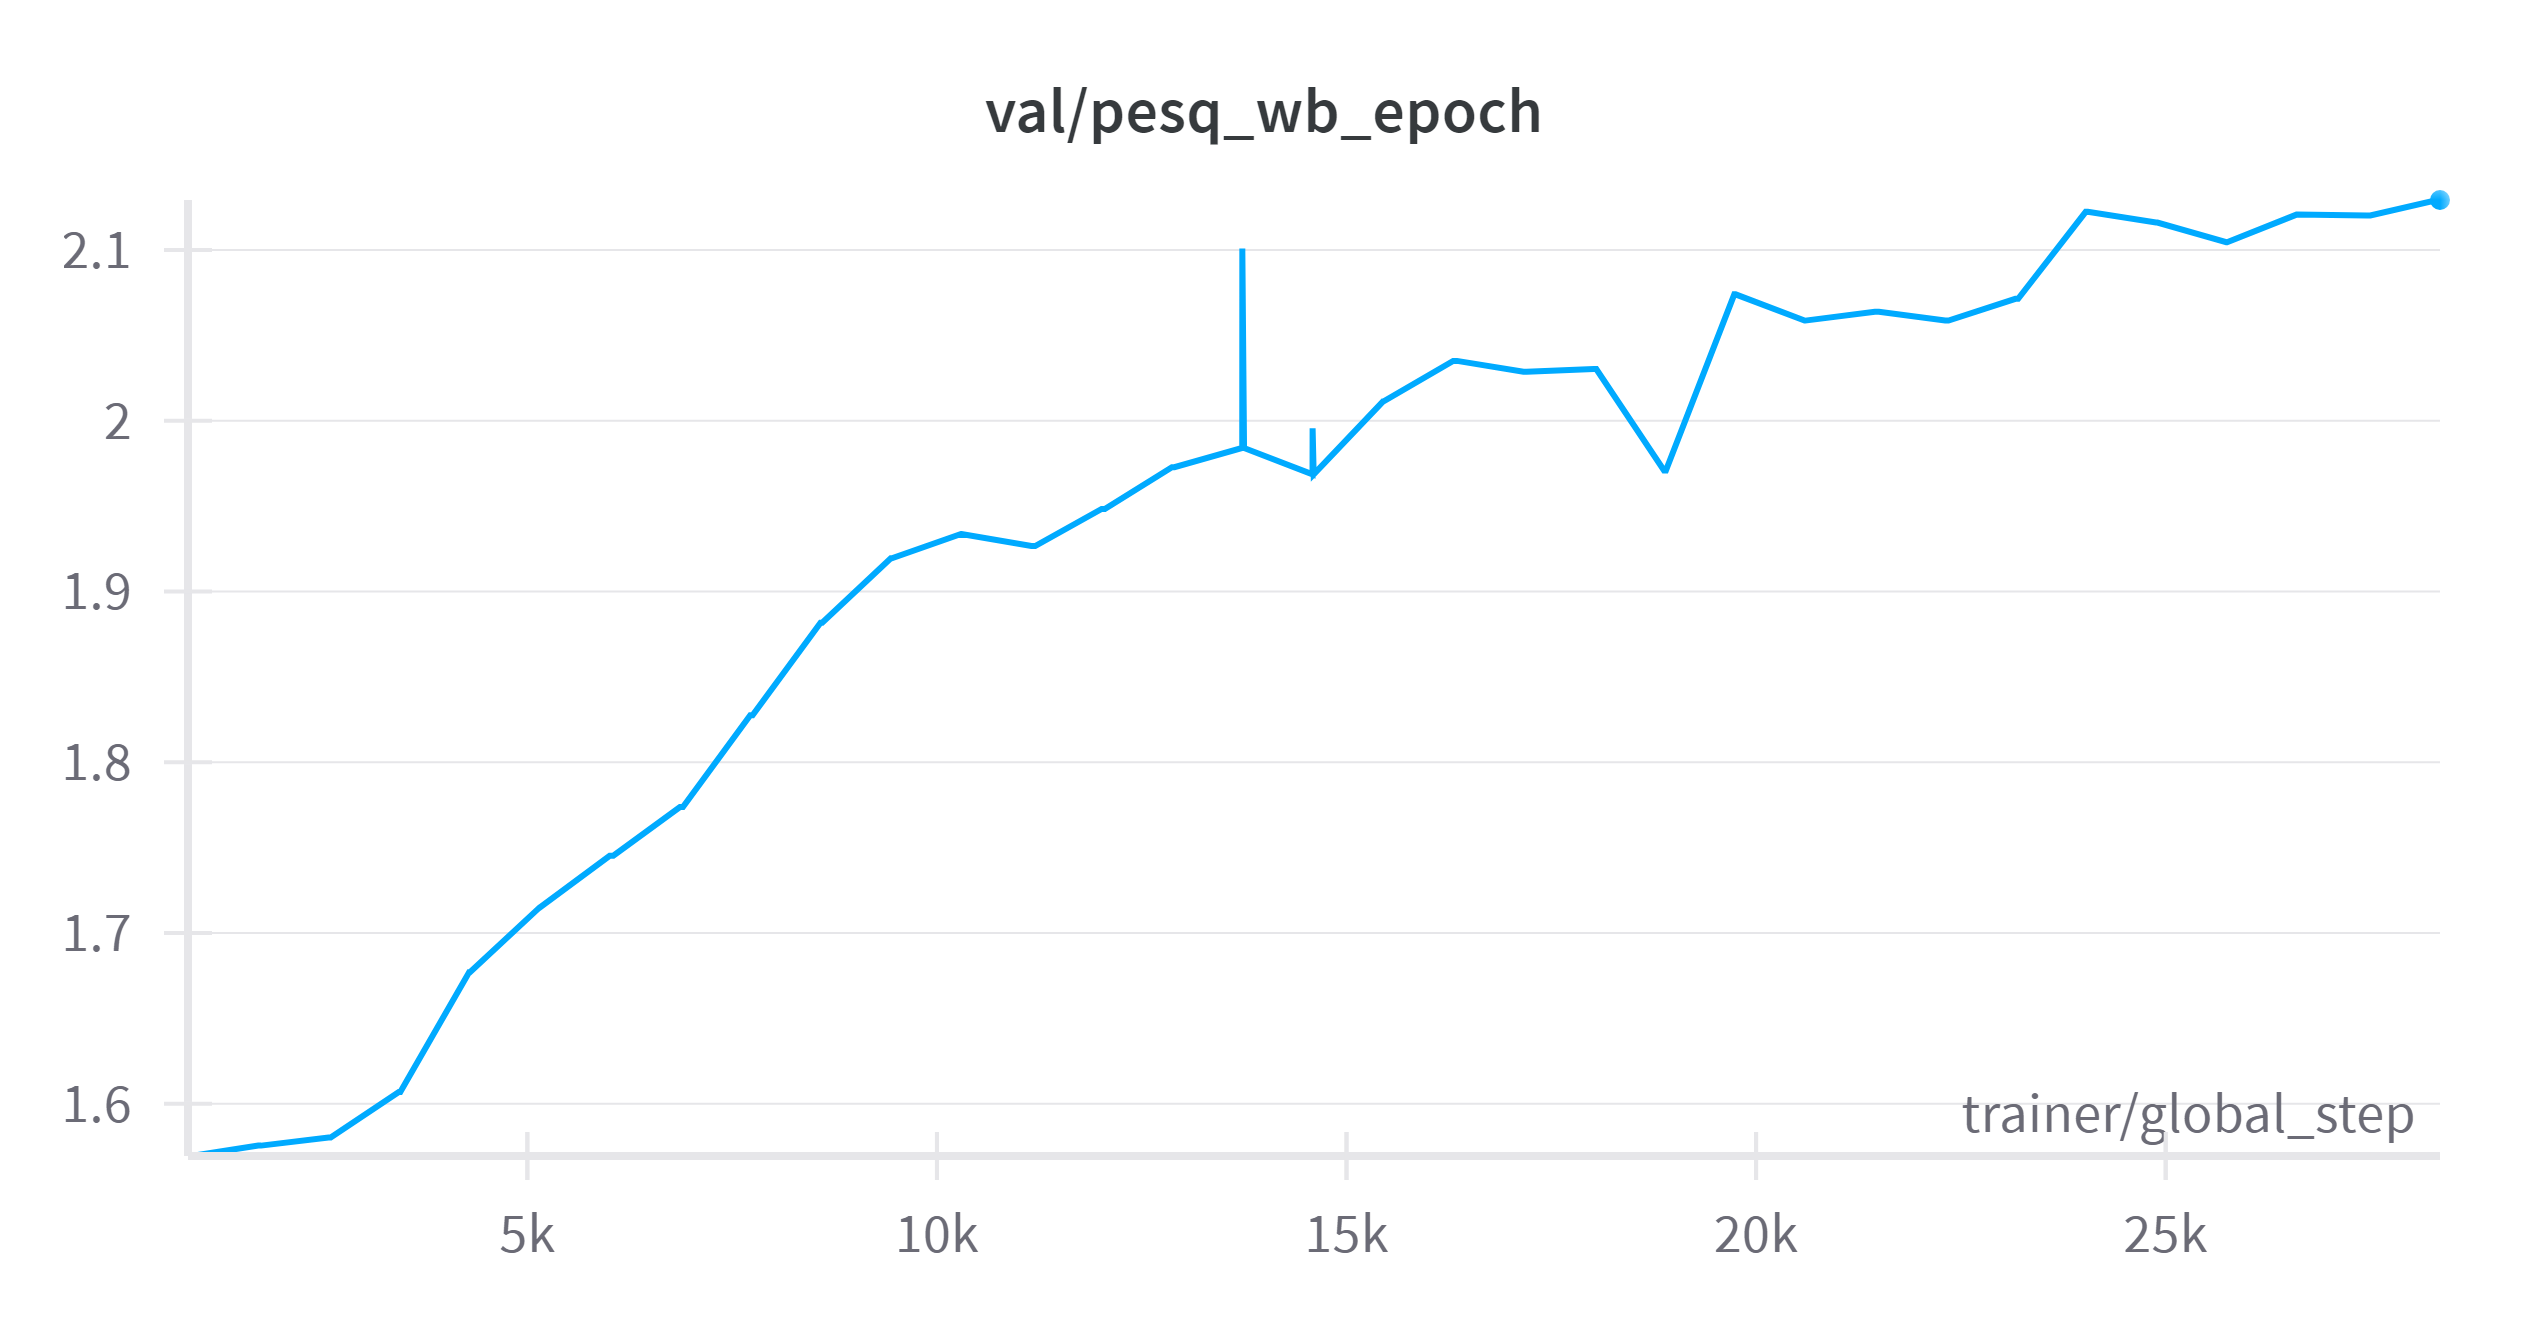
\includegraphics[width=1\linewidth]{images/experiments/denoiser/denoiser_DNS100hrs_val_pesq_wb.png}  
    %     \centering\caption{PESQ-WB reported on\\ test set.}
    %     \label{fig:denoiser_val_pesq_wb}
    % \end{subfigure}
    % \begin{subfigure}{.3\textwidth}
    %   \centering
    %   % include fourth image
    %   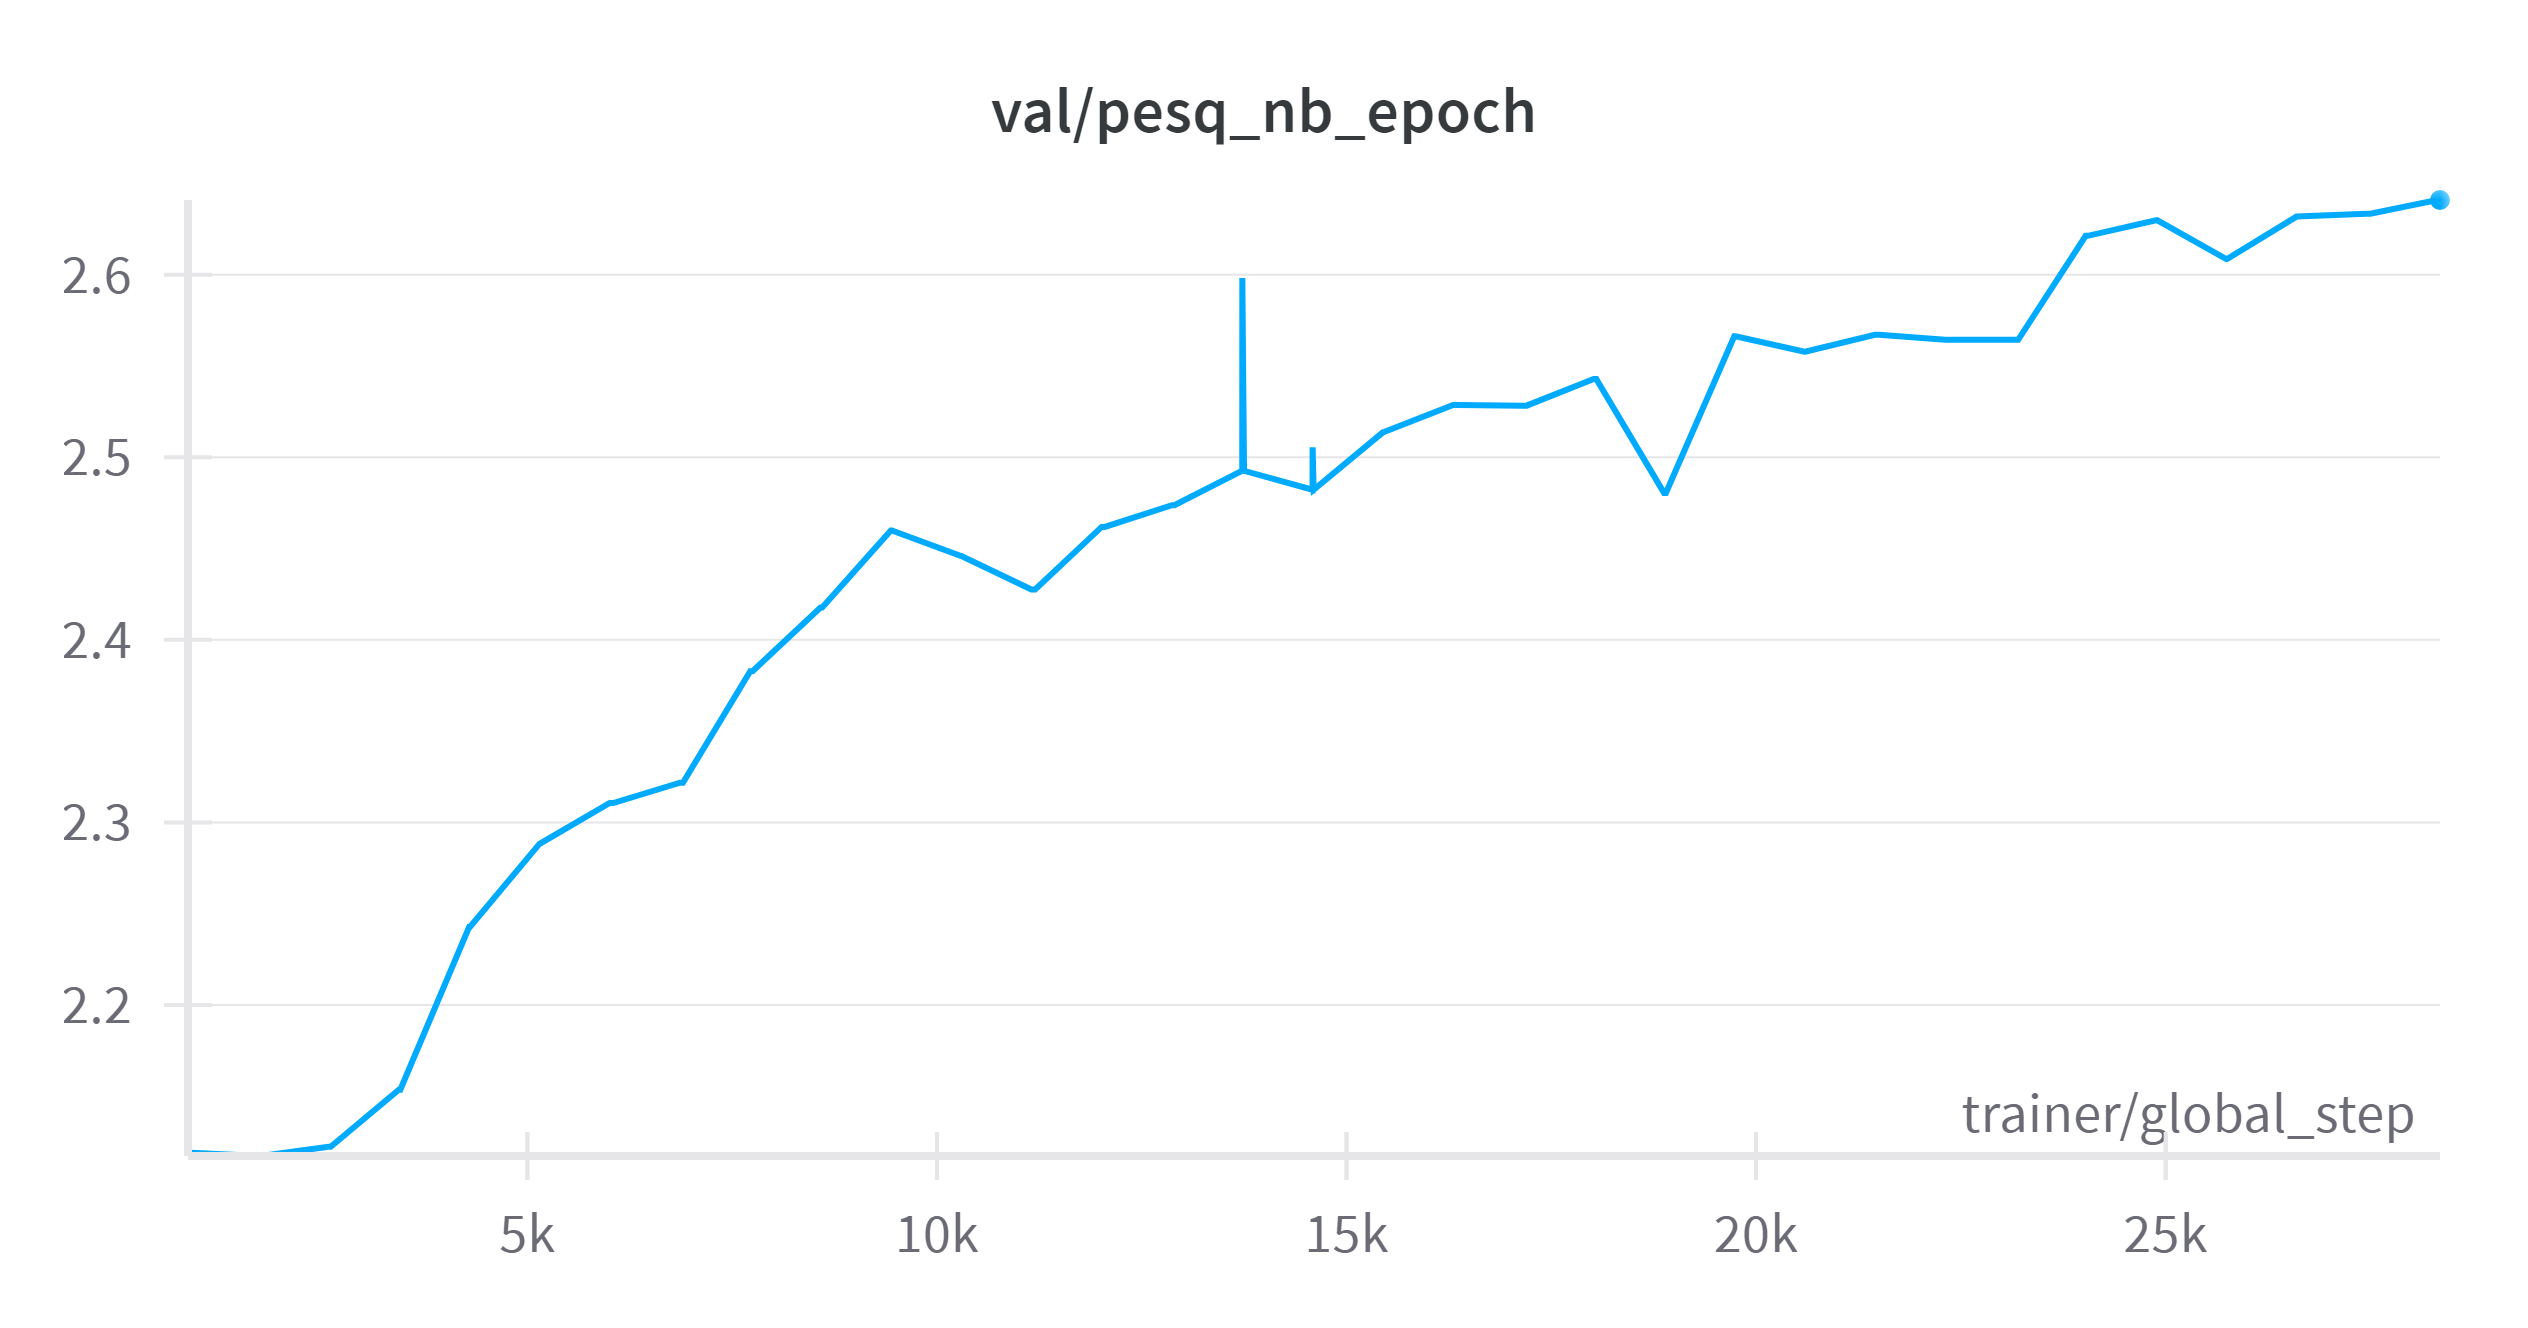
\includegraphics[width=1\linewidth]{images/experiments/denoiser/denoiser_DNS100hrs_val_pesq_nb.png}  
    %   \caption{PESQ-NB reported on\\ test set.}
    %   \label{fig:denoiser_val_pesq_nb}
    % \end{subfigure}
    \caption{Training logs for Denoiser model.}
    \label{fig:denoiser-training}
\end{figure}

\begin{table}[h]
    \centering
    \begin{tabular}{c|c|c}
        \hline
        Metric & Reported & Reproduced \\
        \hline
          
        STOI & 0.95 & 0.934 \\
        % \hline
        PESQ-WB  & 3.07 & 2.129 \\
        % \hline
        PESQ-NB & -- & 2.641 \\
        % \hline
        SIG (MOS) & -- & 3.45 \\
        % \hline
        BAK (MOS) & -- & 4.023 \\
        % \hline
        OVRL (MOS) & -- & 3.172 \\
        \hline
    \end{tabular}
    \caption{Metrics on test set of DNS-2020 dataset (without reverb) for Denoiser model.}
    \label{tab:denoiser-test}
    
\end{table}